\label{sec:ingestaodosdados}

O escopo deste trabalho foi motivado por um projeto de extensão realizado no CEFET-RJ em parceria com a Embratur, cujo objetivo era identificar os destinos brasileiros mais procurados por turistas internacionais. Durante a execução desse projeto, foi observada uma dificuldade relacionada à coleta e integração de dados provenientes de diferentes sites de agências de viagem, os quais apresentam estruturas, formatos distintos.

Entretanto, este Trabalho de Conclusão de Curso não foi desenvolvido para atender às demandas da Embratur nem constitui uma continuidade direta do referido projeto de extensão. O projeto foi utilizado apenas como fonte de inspiração para a definição do problema de pesquisa, fornecendo um contexto prático para a investigação proposta. Além disso, o autor deste trabalho não participou do projeto de extensão mencionado, e a solução apresentada neste TCC foi concebida e desenvolvida de forma independente, com metodologia e escopo próprios.

Para a construção do \textit{pipeline} de dados, foram mapeadas e extraídas informações de dez websites internacionais, de diferentes países, que oferecem pacotes de viagem e passagens aéreas com destino ao Brasil. Essa diversidade de fontes enriquece o conjunto de dados, permitindo uma análise comparativa mais ampla e detalhada. Contudo, essa variedade também impôs desafios significativos, especialmente em relação à diferentes moedas e idiomas. A extração de dados exigiu que os scripts fossem adaptados para lidar com diferentes moedas (Euros, Libras, Dólares americanos e Dólares chilenos) e idiomas (alemão, espanhol, francês e inglês), garantindo que os dados brutos fossem coletados de forma consistente, apesar das variações. Foram desenvolvidos dez scripts para cada site escolhido: Bleu Selectour (França), Comptoir Des Voyages (França), Ikarus Tours (Alemanha), Jetmar (Uruguai), Journey Latin America (Reino Unido), Newmarket Holidays (Reino Unido), Panamericana Turismo (Chile), Sol Férias (Portugal), Transalpino (Portugal) e Turismo Costanera (Chile).

O foco principal do trabalho é a avaliação de ferramentas de código aberto, analisando seu impacto direto na escalabilidade e no desempenho da solução. A metodologia empregada aborda os principais desafios na elaboração da arquitetura, desde a extração de dados dinâmicos até o processamento e armazenamento eficientes. Em suma, este estudo de caso serve como um guia prático para a construção de soluções de dados eficientes, provando que é possível desenvolver sistemas de alta \textit{performance} utilizando um ecossistema de ferramentas acessíveis e flexíveis. 

\section{Tecnologias Utilizadas}

As ferramentas que compõem este \textit{pipeline} foram escolhidas de forma deliberada, seguindo um critério central: selecionar \textbf{uma representante de cada categoria} identificada na literatura revisada, conforme sistematizado na Tabela~\ref{tab:ferramentas_open_source} \cite{mbata2024survey}. O objetivo foi demonstrar a integração entre categorias complementares, ingestão, armazenamento analítico embutido, transformação ELT, orquestração e visualização, utilizando exclusivamente ferramentas open source.

\begin{itemize}
    \item \textbf{Selenium} (\textit{web scraping}/ingestão): Representa a categoria de aquisição de dados dinâmicos. Frente a alternativas como o \textbf{Apache NiFi}, citado na literatura para fluxos de ingestão contínua, o Selenium foi escolhido por sua capacidade de simular interações humanas em páginas com JavaScript, requisito indispensável para os dez sites monitorados. O NiFi é mais adequado a pipelines de dados estruturados e APIs; para raspagem de HTML dinâmico com autenticação visual e paginação interativa, o Selenium é a solução consolidada \cite{mbata2024survey}.

    \item \textbf{DuckDB} (armazenamento analítico embutido/\textit{raw}): Representa a categoria de banco de dados embutido para análise local. Em relação ao \textbf{Pandas}, amplamente usado para manipulação tabular em memória, o DuckDB supera a limitação de carregar todos os dados na RAM, processando diretamente do disco com arquitetura colunar, crucial para médios volumes de dados. Frente ao \textbf{Apache Spark}, ideal para clusters distribuídos de \textit{petabytes}, o DuckDB é mais adequado ao escopo do projeto: não requer infraestrutura de servidores, elimina custos operacionais e integra-se nativamente ao Python \cite{gargouri2026multi}.

    \item \textbf{dbt} (transformação ELT): Representa a categoria de ferramentas de transformação declarativa. Diferentemente de scripts ETL avulsos em Python ou do uso direto de stored procedures, o dbt implementa SQL versionado com testes automáticos, documentação integrada e suporte à arquitetura Medallion, alinhando-se diretamente ao paradigma ELT discutido no Capítulo~2. Foi escolhido em detrimento de alternativas como \textbf{Apache Spark} para transformações (que exigiria infraestrutura distribuída desproporcional ao volume de dados) ou \textbf{AWS Glue} (solução proprietária de nuvem) \cite{gargouri2026multi, mbata2024survey}.

    \item \textbf{PostgreSQL} (\textit{data warehouse} analítico): Representa a categoria de banco relacional como destino central do pipeline. Comparado ao \textbf{MySQL}, o PostgreSQL oferece conformidade mais rigorosa com o padrão SQL, tipos de dados avançados e melhor suporte a cargas analíticas complexas com múltiplas conexões simultâneas, necessárias para que o dbt, o Airflow e o Superset operem em paralelo sobre o mesmo banco \cite{figueira2025arquitetura, gargouri2026multi}.

    \item \textbf{Apache Airflow} (orquestração): Representa a categoria de orquestração e gerenciamento de fluxo de trabalho. Frente ao \textbf{Apache NiFi}, que também suporta orquestração além de ingestão, o Airflow é superior para pipelines orientados a tarefas Python com dependências complexas, pois permite definir DAGs como código, oferece interface web completa de monitoramento e é o padrão de mercado para orquestração de pipelines ELT \cite{mbata2024survey}. O NiFi é mais adequado ao fluxo contínuo de dados em tempo real; o Airflow, ao agendamento e coordenação de tarefas interdependentes. 

    \item \textbf{Apache Superset} (visualização e BI): Representa a categoria de Business Intelligence. Em relação a alternativas open source como \textbf{Metabase} e \textbf{Apache Zeppelin}, o Superset oferece maior riqueza de tipos de gráfico, suporte nativo a filtros cruzados entre painéis e conexão direta via SQLAlchemy com o PostgreSQL \cite{figueira2025arquitetura, mbata2024survey}. Frente a ferramentas proprietárias como Tableau e Power BI, elimina custos de licenciamento mantendo capacidade analítica equivalente para o perfil de uso deste projeto.

    \item \textbf{Docker/Docker Compose} (infraestrutura e conteinização): Representa a categoria de infraestrutura reprodutível. O Docker foi escolhido por garantir que o ambiente completo do pipeline, scrapers, banco de dados, Airflow, dbt e Superset, possa ser reproduzido em qualquer máquina com um único comando, eliminando conflitos de dependências entre os serviços \cite{figueira2025arquitetura, gargouri2026multi}.
\end{itemize}

O processo de construção do pipeline de dados foi integralmente desenvolvido em Python, uma linguagem de programação cuja aplicabilidade em automação e no ecossistema de processamento de dados a torna uma escolha robusta para projetos de ED.

A Figura~\ref{fig:arquitetura} apresenta a visão geral da arquitetura do pipeline desenvolvido. O fluxo de dados percorre cinco etapas: (1) extração dos dados de dez sites internacionais via Selenium e Python; (2) armazenamento dos dados brutos no DuckDB, que atua como repositório temporário (\textit{raw}); (3) transformação e padronização dos dados pelo dbt; (4) consolidação no PostgreSQL, que serve como \textit{data warehouse} analítico; e (5) visualização por meio do Apache Superset. O Apache Airflow orquestra todas as etapas de forma automatizada, e toda a infraestrutura é conteinerizada via Docker Compose, garantindo a reprodutibilidade do ambiente.

\begin{figure}
    \centering
    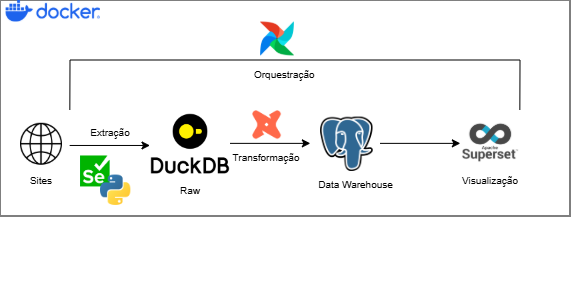
\includegraphics[width=1.0\linewidth]{img/arquitetura.png}
    \caption{Arquitetura completa do pipeline de dados}
    \label{fig:arquitetura}
\end{figure}

Para a fase crucial de aquisição e extração de conteúdo dinâmico (\textit{web scraping}), a ferramenta central adotada foi o \textbf{Selenium WebDriver}. Este framework de automação de navegadores serviu como a espinha dorsal da solução, simulando o comportamento de um usuário real (como cliques, rolagem de página e interações complexas com elementos de interface, utilizando recursos da biblioteca que permitem simular ações do mouse e selecionar opções em menus suspensos). Sua capacidade de lidar com interações complexas garante a extração de dados de fontes que demandam alta flexibilidade de acesso.

Uma vez extraídos, os dados brutos foram imediatamente direcionados para o \textbf{DuckDB}, que atuou como repositório temporário de alto desempenho. O DuckDB é um sistema de banco de dados relacional e analítico que se destaca por sua arquitetura embutida, ou seja, ele funciona diretamente dentro do programa que o utiliza, sem a necessidade de instalar ou manter um servidor de banco de dados separado. Essa característica simplifica a arquitetura do projeto e minimiza os custos indiretos associados à complexidade operacional e manutenção de um componente dedicado.

Após a ingestão inicial, os dados brutos foram migrados para o \textbf{PostgreSQL}, um sistema de gerenciamento de banco de dados relacional open source que atua como o DW analítico do projeto. Diferentemente do DuckDB, o PostgreSQL opera no modelo cliente-servidor, o que siganifica que ele funciona como um serviço independente ao qual múltiplas ferramentas podem se conectar simultaneamente, uma característica essencial para a integração com as demais tecnologias do pipeline. Sua robustez, ampla conformidade com padrões SQL e mais de 35 anos de desenvolvimento ativo o consolidam como uma das soluções open source mais confiáveis para cargas analíticas.

Para a camada de transformação dos dados, foi adotado o \ac{dbt}, uma ferramenta open source que implementa o paradigma de transformação como código (\textit{transformation as code}). Em termos práticos, isso significa que todas as regras de limpeza, padronização e reorganização dos dados são escritas em SQL, a linguagem padrão para consultas em bancos de dados, e armazenadas em arquivos versionáveis, da mesma forma que se versiona o código de um software. O dbt opera exclusivamente sobre os dados já carregados no PostgreSQL, alinhando-se à abordagem ELT discutida no Capítulo 2. Seu sistema integrado de testes automáticos e documentação agrega uma camada de qualidade e governança que seria difícil de replicar com scripts avulsos.

A orquestração de todo o pipeline, desde a execução dos scripts de web scraping até a materialização dos modelos dbt, foi confiada ao \textbf{Apache Airflow}, uma plataforma open source de gerenciamento de fluxos de trabalho. O Airflow permite a definição de pipelines como código Python, utilizando o conceito de \acs{dags}, que são grafos direcionados sem ciclos nos quais cada nó representa uma tarefa a ser executada e as setas entre eles definem a ordem de execução, ou seja, qual tarefa precisa terminar antes que a próxima comece. Sua interface web oferece visibilidade completa sobre o histórico de execuções, registros detalhados de cada etapa e mecanismos automáticos de reexecução em caso de falha, garantindo a observabilidade e a resiliência do pipeline em produção.

Por fim, a disponibilização dos dados transformados para análise visual foi realizada por meio do \textbf{Apache Superset}, uma plataforma open source de \acs{bi} que permite a criação de painéis interativos (\textit{dashboards}) e a exploração de dados via consultas SQL. O Superset conecta-se nativamente ao PostgreSQL e se posiciona como uma alternativa direta a ferramentas proprietárias como Tableau e Power BI, sem custos de licenciamento.

Em paralelo, o processamento e a qualidade dos dados foram aprimorados pelo uso estratégico de bibliotecas nativas do Python. A biblioteca de expressões regulares foi essencial na etapa de transformação para identificar e extrair padrões específicos dentro de textos, como valores monetários e durações de viagem que estavam misturados em frases descritivas. Adicionalmente, bibliotecas auxiliares foram integradas ao pipeline para gerenciar a organização dos arquivos e enriquecer os dados com informações temporais (como a data e hora da coleta), garantindo a rastreabilidade e a consistência do conjunto de dados final.

\section{Tentativa com a ferramenta Browser Use}

Antes de iniciar a abordagem manual com o Selenium, foi explorada a possibilidade de usar ferramentas de inteligência artificial para a extração de dados. A ferramenta Browser Use, que atua como um agente de navegação autônomo, prometia uma alternativa mais intuitiva e menos dependente de seletores CSS fixos, ao permitir a automação de tarefas online em linguagem natural. Essa abordagem era perfeitamente alinhada com a premissa do trabalho, que busca soluções \acs{open_source} e flexíveis. O agente foi configurado para usar o modelo de linguagem Mistral, que rodou localmente via Ollama e foi orquestrado com a biblioteca LangChain.

O Mistral 8x7B é um Grande Modelo de Linguagem (\ac{llm}) notável por sua arquitetura Mixture of Experts (MoE), sendo composto por oito módulos especialistas, cada um contendo sete bilhões de parâmetros. Essa estrutura é projetada para especializar-se em diferentes tipos de tarefas e está na vanguarda da pesquisa em aprendizado multimodal, visando aprimorar a integração e o processamento de dados de texto, imagem e áudio.

A tentativa demonstrou que o \textit{Browser Use} é funcional. O modelo conseguia interagir com as páginas e extrair informações, validando a promessa de que é possível automatizar o processo com comandos de alto nível. No entanto, essa abordagem enfrentou uma limitação técnica significativa: o processamento local do modelo de IA. A execução do Mistral via Ollama se mostrou extremamente intensiva em termos de recursos computacionais, sobrecarregando a máquina utilizada para o projeto.

Os testes foram realizados em um computador DESKTOP-I0H93GR, equipado com um processador \textit{AMD Ryzen 7 4800HS with Radeon Graphics} (2,90 GHz), 16 GB de memória RAM (15,4 GB utilizáveis) e sistema operacional Windows 10 de 64 bits. Apesar de possuir boas especificações para tarefas gerais de desenvolvimento, a execução local do modelo exigiu recursos acima da capacidade disponível, resultando em lentidão significativa e, em alguns casos, no desligamento completo do computador devido à alta demanda de CPU e memória RAM.

Essa limitação inviabilizou a continuidade do projeto com essa arquitetura, evidenciando a necessidade de recursos computacionais mais robustos ou da adoção de uma abordagem baseada em infraestrutura em nuvem para o processamento de modelos de linguagem de grande porte.

Essa experiência reforça a importância de considerar o custo operacional e os requisitos de infraestrutura ao escolher as ferramentas para um \textit{pipeline} de dados, especialmente em projetos que buscam a acessibilidade e a eficiência. A tentativa, embora não tenha sido bem-sucedida em termos de implementação prática devido às limitações de \textit{hardware}, serviu como uma valiosa lição sobre as barreiras que ainda existem para o uso de soluções de IA em ambientes de baixo custo, destacando que essa abordagem é promissora para o futuro, desde que haja um \textit{hardware} mais potente à disposição.